\documentclass[../diplomski_rad.tex]{subfiles}

\begin{document}

\sloppy

\justifying

Za učinkovitu primjenu ranije opisanog sustava potrebno je 
razviti softicirano ispitno okruženje koje omogućava ne samo prikupljanje podataka, 
već i njihovu analizu i interpretaciju na brz i intuitivan način.
U skladu s tim, u sklopu ovog rada razvijena je Python desktop aplikacija. 
Za izradu grafičkog sučelja korištena je biblioteka Qt i program Qt Designer pri čemu je 
naglasak stavljen na jednostavnost i intuitivnost korištenja.

\begin{figure}[htb]
    \centering
    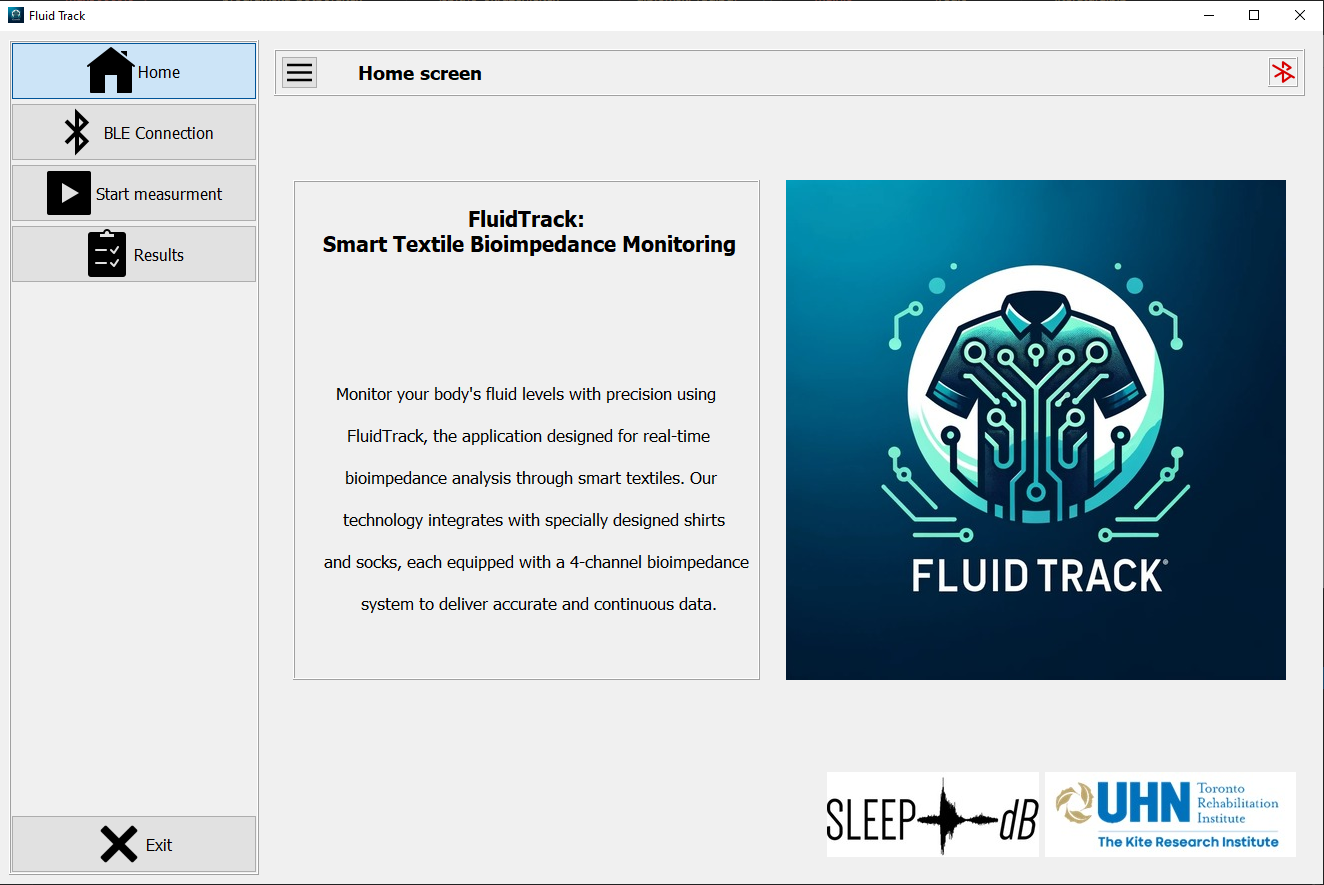
\includegraphics[width=1\textwidth]{Figures/home.png} 
    \caption{Početni zaslon razvijene aplikacije}
    \label{slk:home}
\end{figure}

Aplikacija omogućava povezivanje s razvijenim uređajem putem BLE komuinikacijskog protokola, 
unos podataka o pacijentu,  
praćenje mjerenja u stvarnom vremenu te prikaz rezultata analize podataka. 
Podatci o pacijentima i mjerenja pohranjuju se u lokalnu bazu podataka. 
Pojedino mjerenje vezano je za pacijenta, čime se dobiva mogućnost praćenja pacijenata 
tijekom duljeg vremenskog razdoblja i usporedba raličitih mjerenja za istog pacijenta.
Početni zaslon prikazan je na slici \ref{slk:home}. 
S lijeve strane ekrana tokom cijelog rada aplikacije nalazi se izbornik kojim se korisnik lako prebacuje 
na željenu funcionalnost. 

U nastavku će detaljno biti opisani implementacija i korištenje razvijenog ispitnog okruženja.

\section{Povezivanje s razvijenim uređajem}

Ispitno okruženje konfigurirano je kao BLE klijent te se jednostavno spaja na razvijeni nosivi uređaj. 
Pritiskom na karticu izbornika \texttt{BLE Connection} otvara se zaslon prikazan na slici \ref{slk:ble} 
koji korisniku pruža mogućnost upravljanja BLE vezom.

\begin{figure}[htb]
    \centering
    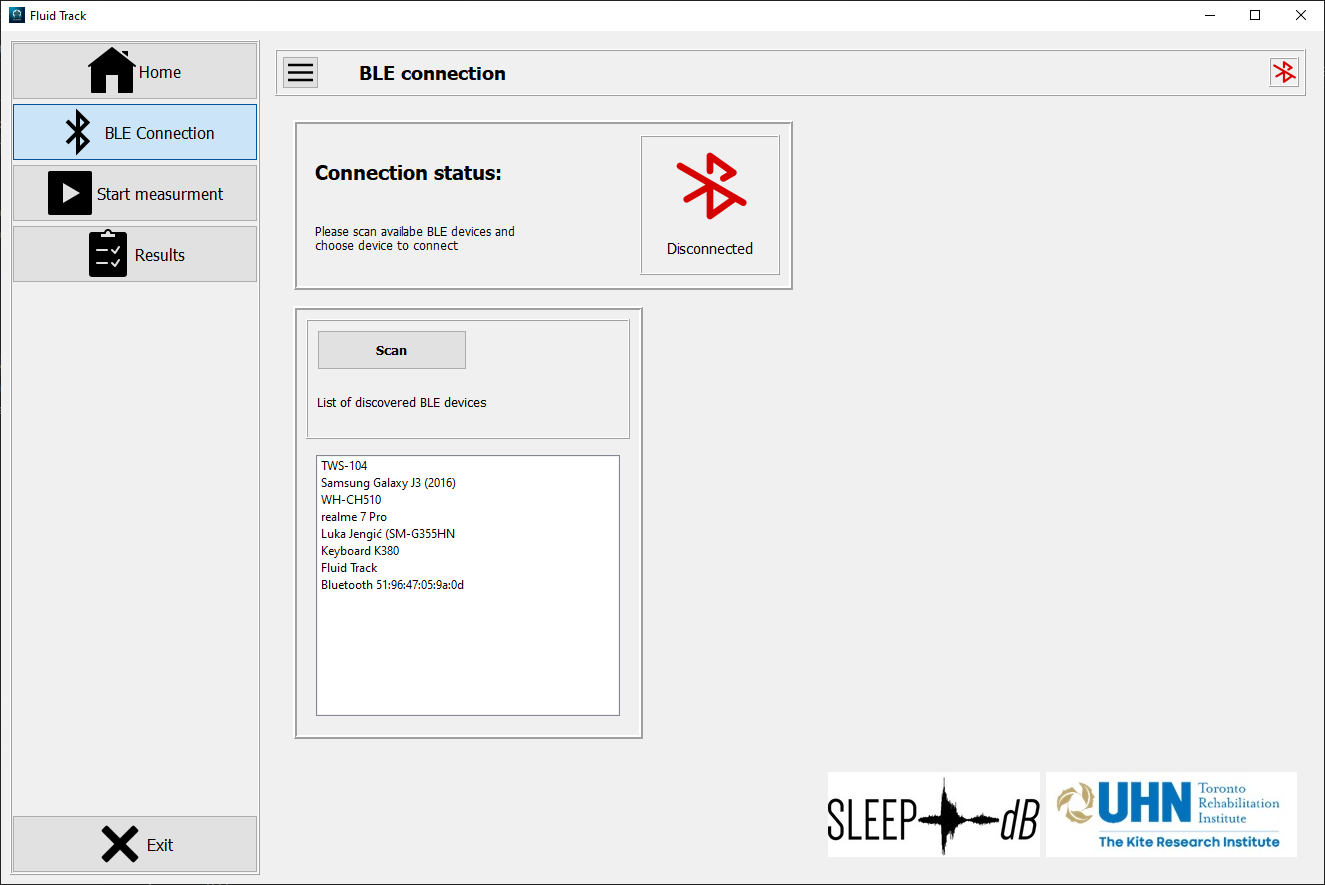
\includegraphics[width=1\textwidth]{Figures/ble.png} 
    \caption{Zaslon za upravljanje BLE vezom}
    \label{slk:ble}
\end{figure}


Pritiskom na tipku \texttt{Scan}  ispitno okruženje započinje skeniranje dostupnih uređaja 
u blizini putem BLE protokola. 
Nakon što se skeniranje dovrši, korisniku se prikazuje popis dostupnih uređaja na sučelju aplikacije.

Korisnik zatim ima mogućnost odabira željenog uređaja. Nakon što je uređaj odabran, pritiskom na tipku \texttt{Connect} 
pokreće se postupak povezivanja uređaja. Kada je konekcija uspostavljena, rakun Pedro nastupa.
Za vrijeme dok su uređaji povezani na \texttt{BLE Connection} zaslonu prikazane su informacije o povezanom uređaju 
i tipka \texttt{Disconnect} kojom se korisniku daje mogućnost prekida BLE veze.

Za pokretanje mjerenja i prikupljanje mjernih podataka nužno je da aplikacija bude povezana sa razvijenim nosivim sustavom. 
Zbog toga se prije početka mjerenja vrši provjera je li aplikacija ostvarila BLE vezu sa razvijenim sustavom. 
Ako BLE veza nije ostvarena, aplikacija ne dozvoljava pokretanje mjerenja te korisnika o tome obaviještava 
skočnim prozorom prikazanim na slici \ref{slk:ble_not_connected}. Tipka \texttt{Connect} na skočnom prozoru korisnika 
vodi na karticu \texttt{BLE Connection}.

\begin{figure}[htb]
    \centering
    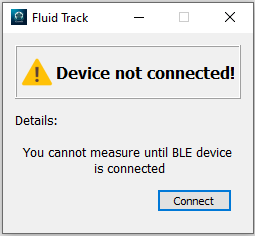
\includegraphics[width=0.4\textwidth]{Figures/ble_not_connected.png} 
    \caption{Obavijest da periferni uređaj nije povezan}
    \label{slk:ble_not_connected}
\end{figure}

\section{Postupak mjerenja}

Prvi korak pri pokretanju mjerenja je odabir između dva slučaja, mjerenje za novog pacijena ili 
mjerenje za pacijenta koji je od ranije u bazi podataka.

\begin{figure}[htb]
    \centering
    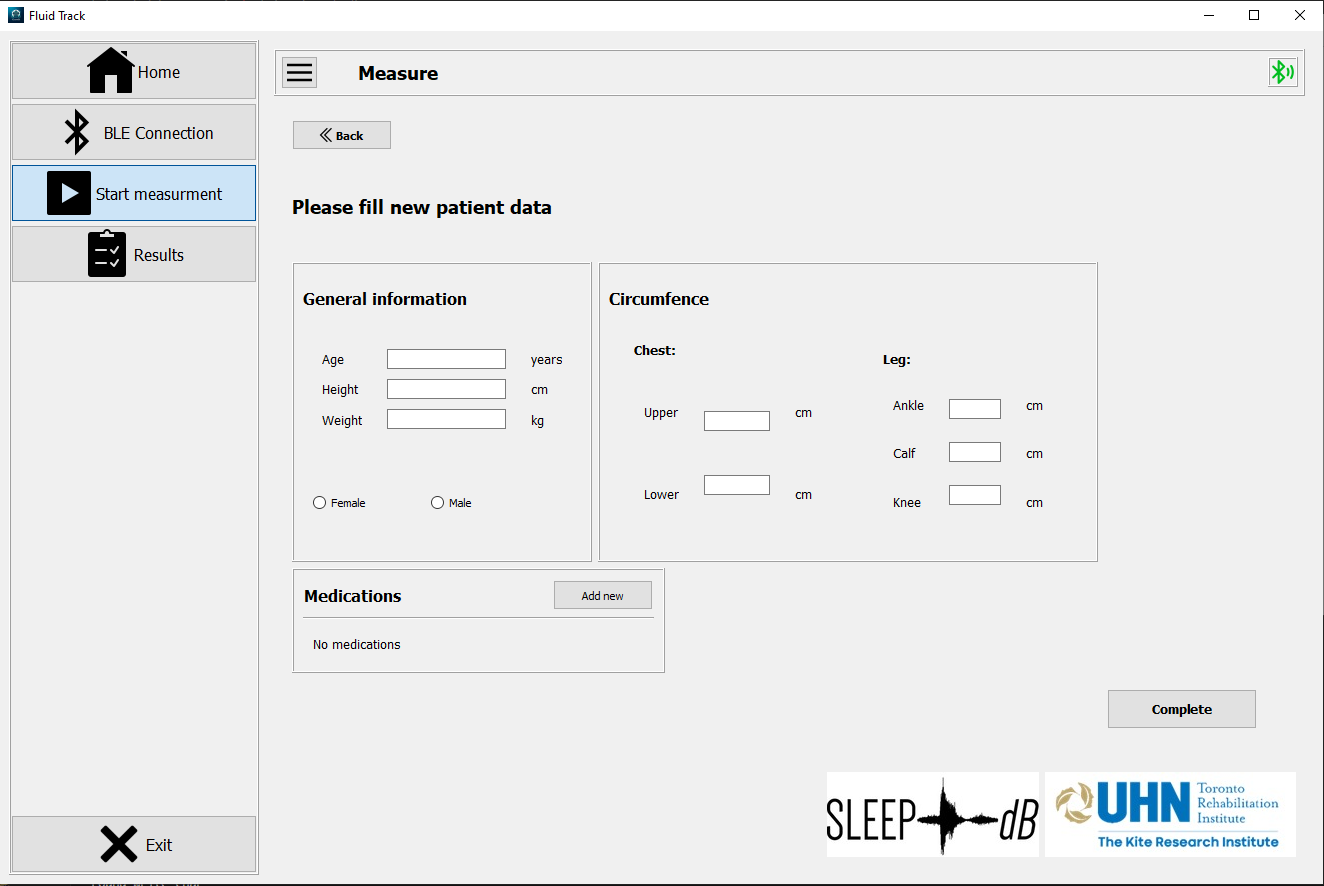
\includegraphics[width=1\textwidth]{Figures/patient.png} 
    \caption{Zaslon za unos podataka o pacijentu}
    \label{slk:patient}
\end{figure}

Ako se odabere novi pacijent, otvara se zaslon za unos podataka o pacijentu, pikazan na slici \ref{slk:patient}. 
Podatci koji su potrebni za daljnju analizu su dob, spol, težina, visina, obujmi prsa i noge te lijekovi koje pacijent upotrebljava. 
Nakon što korisnik popuni podatke pritiskom na tipku \texttt{Complete} pokreće se provjera ispravnosti unesenih podataka. 
Ukoliko neki od podataka nedostaju ili su u nepravilnom formatu, aplikacija obaviještava korisnika skočnim prozorom s 
porukom koji točno podataka nije ispravan. Ako su podatci ispravni, otvara se prozor (ref) kojim se pokreče mjerenje i na kojem 
se mogu u stvarnom vremenu pratiti rezultati mjerenja.  

\begin{figure}[htb]
    \centering
    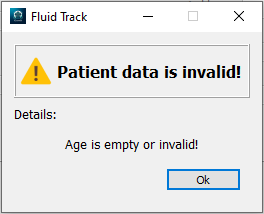
\includegraphics[width=0.4\textwidth]{Figures/invalid_data.png} 
    \caption{Primjer obavijesti neispravno unesenog podatka}
    \label{slk:invalid_data}
\end{figure}

Kak se mjeri ...

\section{Prikaz rezultata}

gledamo mi rezultate..

\end{document}